\section{Comportamento}
Il comporamento del sito è gestito lato server da PHP e lato client da JavaScript.

\subsection{JavaScript}
Abbiamo usato un unico file JavaScript nominato checkForm.js, contenente principalmente funzioni che svolgono controlli sull'input delle form.
Di seguito riportiamo le funzioni con una breve spiegazione:

\begin{itemize}
	\item \textbf{validateForm(): } esegue un controllo lato client dell'input della form. Viene chiamata in tutte le pagine che contengono delle form per l'inserimento o la modifica dei dati lato admin e nelle pagine di login e registrazione lato utente.
	Per facilitare eventuali aggiunte di campi input nel sito, la funzione si appoggia all'array \texttt{dettagliForm} contenente come chiavi gli id dei campi input a cui vengono associati array contenenti le espressioni regolari per la verifica dell'input e i corrispondenti messaggi d'errore.
	La funzione procede chiamando \texttt{validateInput(input)} per ogni elemento di \texttt{dettagliForm} trovato nella pagina di invocazione, prosegue chiamendo \texttt{checkChecked()} ed infine ritorna un valore booleano in base all'esito dei controlli effettuati; \\

	\item \textbf{validateInput(input): } effettua il controllo del campo input. Nel caso sia già presente un messaggio (di errore o di conferma del corretto inserimento), lo rimuove. Gestisce in seguito i casi limite, non gestibili tramite l'array di supporto: campi input di tipo file o data, il campo \texttt{repeatedpassword} e i campi opzionali. Effettua quindi il controllo dei restanti campi input sfruttando le espressioni regolari presenti in \texttt{dettagliForm} e procede ritornando il valore ricevuto dall'invocazione di \texttt{showMessage(input,stato)}; \\

	\item \textbf{showMessage(input, stato): } crea un messaggio che comunica all'utente se l'input inserito è corretto o meno. Abbiamo deciso di fornire 2 meccanismi di feedback all'utente, presentando sia un messaggio testuale che una colorazione del bordo del campo input, in questo modo possiamo facilitare la compilazione delle form a tutte le classi di utenti. \\

	\item \textbf{checkPassword(): } controlla che gli input in \texttt{password} e in \texttt{repetedpassword} siano uguali e invoca opportunamente \texttt{showMessage(input,stato)}; \\

	\item \textbf{checkChecked(): } effettua un controllo dei campi checkbox e radio sfruttando l'array di supporto \texttt{spuntabili} in modo analogo a \texttt{validateForm()}. Crea un array contenente coppie chiave-valore nella forma: id del campo input, valore booleano (che indica se il rispettivo campo input è stato spuntato). Tale array viene poi fornito come parametro a \texttt{showMessageCheckbox(sezioni)}; \\

	\item \textbf{showMessageCheckbox(sezioni): } opera in modo analogo a \texttt{showMessage(input, stato)}, creando però dei messaggi che comunicano all'utente se i campi input (di tipo checkbox o radio) sono stati spuntati o meno; \\

	\item \textbf{handleClick(): } fa comparire/scomparire il campo'\texttt{Gioco trattato}" se viene selezionata/deselezionata la categoria\texttt{Giochi}' in \texttt{Tipologia} nella form per l'inserimento di una notizia; \\

	\item \textbf{removeNoJs(): }  viene invocata al completamento del caricamento della pagina, rimuove la classe'no-js" dal tag \texttt{<html>}. Tale classe è stata utilizzata per la definizione di alcune regole \texttt{css} che gestiscono la casistica in cui JavaScript è disattivato. Ad esempio nel caso del menù principale nella versione mobile, con JS disattivato, viene rimosso il pulsante e viene mostrata la tendina aperta; \\

	\item \textbf{checkNotEmpty(id): } controlla che il campo \texttt{input} con id ='id" non sia vuoto o composto da spazi; \\

	\item \textbf{responsiveMenu(): } gestisce l'apertura e chiusura del menù a tendina nella versione mobile.
	E' associata ad un evento \texttt{onclick}, scelto perchè gestisce anche l'evento \texttt{ontouch} per dispositivi mobile.
	Il pulsante è situato nel top-right della pagina, dove è più facilmente raggiungibile da un utente mobile; \\

	\item \textbf{preparaFiltri(): } viene chiamata al completamento del caricamento della pagina \texttt{Giochi}. Gestisce l'evento onclick dei button tramite event delegation nel \texttt{div} con classe'container". All'evento onclick di un bottone dei filtri di ricerca lascia aperta la tendina contenente i filtri, mentre ad un secondo evento onclick all'interno del'container" la richiude; \\

	\item \textbf{checkAnni(): } effettua un controllo sull'intevallo degli anni di uscita dei videogiochi selezionato nella pagina giochi.
	Inserisce un messaggio d'errore se l'intervallo è inamissibile (es: da 2020 a 2016) e blocca il submit. \\
\end{itemize}




\subsection{BackEnd}
Il backend del server è stato sviluppato con script PHP e database relazionale MariaDB.

\subsubsection{Php}

Gli script che costituiscono il backend si possono suddividere in 3 macro categorie in base alla loro funzione:
\begin{enumerate}
	\item \textbf{modellazione dei dati}.
	\begin{itemize}
		\item comment.php
		\item game.php
		\item image.php
		\item news.php
		\item user.php
	\end{itemize}
	\item \textbf{interazione con il database};
	\begin{itemize}
		\item dbConnection.php
	\end{itemize}
	\item \textbf{creazione e presentazione delle pagine html};
	\begin{itemize}
		\item edit\_gioco.php
		\item edit\_notizia.php
		\item edit\_profilo.php
		\item form\_gioco.php
		\item form\_notizia.php
		\item giochi.php
		\item gioco\_notizie.php
		\item gioco\_recensione.php
		\item gioco\_scheda.php
		\item home.php
		\item lista\_utenti.php
		\item login.php
		\item notizia.php
		\item notizie.php
		\item profilo.php
		\item registrati.php
		\item replacer.php
	\end{itemize}
\end{enumerate}
\paragraph{Modellazione dei dati}
I dati gestiti dal nostro sito sono per la maggior parte classificabili in 5 tipi, illustrati singolarmente nei paragrafi successivi. Per favorire l'ordine all'interno del codice e nella comunicazione dei dati, ogni tipo di viene associato ad una classe.

\subparagraph{Gioco}
Contiene le informazioni riguardanti un gioco e la recensione che lo riguarda.
\subparagraph{Notizia}
Contiene le informazioni riguardanti una notizia.
\subparagraph{Utente}
Contiene le informazioni riguardanti un utente salvato nel sistema, che può essere di tipo amministratore o utente semplice.
\subparagraph{Immagine}
Contiene il percorso di un'immagine salvata nel server e il testo alternativo che la accompagna.
\subparagraph{Commento}
Contiene le informazioni un commento rilasciato da un utente riguardo ad un gioco.

\paragraph{Interazione con il database}
Il file dbConnection.php presenta la classe DBAccess che permette di aprire una connessione verso il database e di effettuare richieste ad esso. Per ognuno dei tipi di dato presentati nel paragrafo precedente sono rese disponibili le seguenti funzionalità:
\begin{itemize}
	\item ottenimento della lista dei dati;
	\item aggiunta di un nuovo dato;
	\item modifica di un dato già presente;
	\item rimozione di un dato già presente. 
\end{itemize}

In aggiunta sono presenti delle specializzazioni di queste operazioni e alcune ulteriori operazioni per l'accesso alle tabelle del database non direttamente rappresentate da una classe, ovvero Prequel\_Sequel, Games\_Consoles e Games\_Genres.

\paragraph{creazione e presentazione delle pagine html}

\subsubsection{Database}


  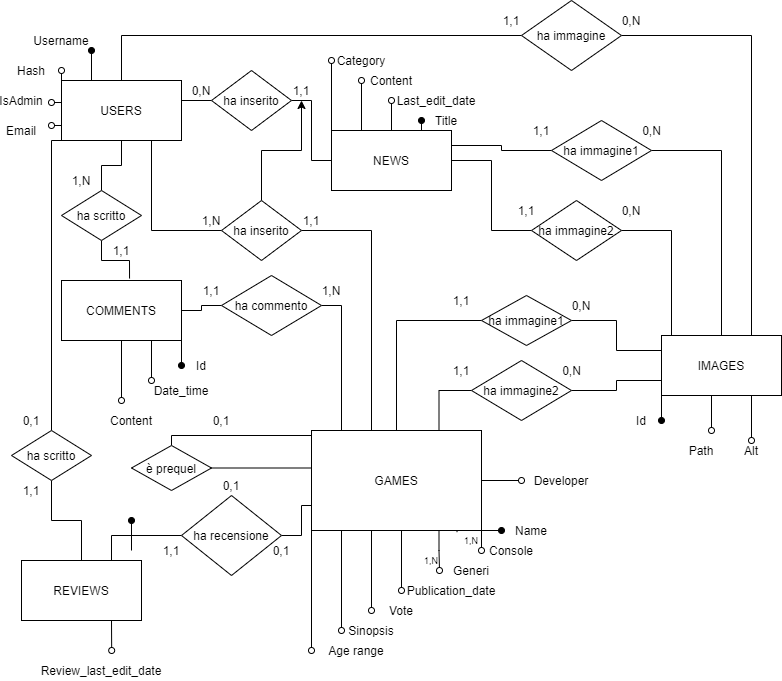
\includegraphics[width=\linewidth]{./img/diagramma_er.png}
  


